\documentclass[11pt,a4paper]{article}
\usepackage[margin=2.3cm]{geometry}
\usepackage{amsmath,amssymb}
\usepackage{graphicx}
\usepackage{booktabs}
\usepackage{xcolor}
\usepackage[font=small,labelfont=bf]{caption}
\usepackage{microtype}
\usepackage{placeins}
\usepackage{braket}
\usepackage[skins,breakable]{tcolorbox}
\usepackage[colorlinks=true,linkcolor=blue!50!black,citecolor=blue!50!black,urlcolor=blue!50!black]{hyperref}
\usepackage[capitalise,nameinlink]{cleveref}
\graphicspath{{../figs/}}
\emergencystretch=3em

\newtcolorbox{finding}[1][]{enhanced,breakable,colback=blue!4,colframe=blue!50!black,
  fonttitle=\bfseries,title={Finding#1}}
\newtcolorbox{definition}[1][]{enhanced,breakable,colback=black!3,colframe=black!45,
  fonttitle=\bfseries,title={Definition#1}}

% model colours, as in make_figs.py (METHOD_COLORS)
\definecolor{ctracked}{HTML}{FF0000}
\definecolor{cfid}{HTML}{0000FF}
\definecolor{cunwrap}{HTML}{CC79A7}
\definecolor{cwrap}{HTML}{56B4E9}
\newcommand{\tracked}{\textcolor{ctracked}{tracked fidelity fit}}
\newcommand{\fidfit}{\textcolor{cfid}{single-time fidelity fit}}
\newcommand{\unwrapped}{\textcolor{cunwrap}{unwrapped phase}}
\newcommand{\wrapped}{\textcolor{cwrap}{wrapped phase}}

\title{Phase branches and near-zeros in the cumulant expansion of a quenched state}
\author{}
\date{28 October 2026}

\begin{document}
\maketitle

\begin{abstract}
For ground states, the infidelity of a restricted Boltzmann machine (RBM) closely follows that of a truncated cumulant expansion of $\log\psi$ with as many terms as the RBM has parameters~\cite{Cortes25}. We ask whether this carries over to real-time dynamics, where $\log\psi$ is complex and its imaginary part is defined only up to $2\pi$. For the transverse-field Ising quench $g=1.5\to0.5$ on an open chain of $L=10$ spins, making the phase continuous in time removes the $2\pi$ wrapping problem, but the expansion fails after $t\approx0.5$. By then hundreds of configurations have nearly vanishing amplitude, and the two branch searches we tried did not make their logarithm compressible. Defining the cumulant coefficients instead by fitting $\exp(\sum_A c_A s^A)$ to $\psi$, and making the coefficients (not the phase) continuous in time, gives a model whose infidelity tracks the RBM infidelity. Its rank correlation with the RBM is $0.98$ over times and hidden-unit densities at $g_f=0.5$, and $0.93$ across runs at fixed time. Over all quenches the model lies a median factor of $3.7$ below the RBM; this factor varies between $1.7$ and $27$ from quench to quench. After $t\approx0.5$ even the RBM state's own cumulants cannot be truncated to as many terms as the RBM has parameters.
\end{abstract}

\begin{figure}[h]
  \centering
  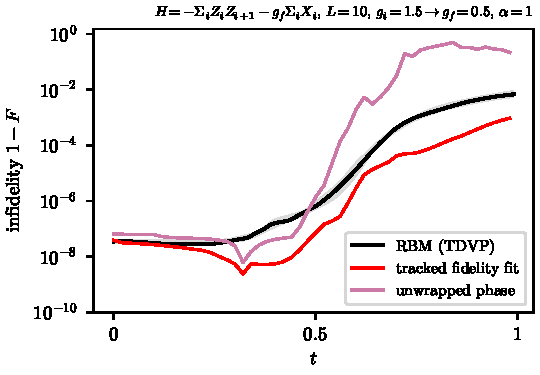
\includegraphics[width=0.46\linewidth]{graphical_abstract.pdf}
  \caption{Main result in one panel. Infidelity $1-F$ with the exact state along the quench $g_i=1.5\to g_f=0.5$ of the transverse-field Ising chain ($L=10$), for an RBM with hidden-unit density $\alpha=1$ and for two cumulant models with the same number $K=120$ of complex parameters. Black: RBM time evolution (median over five trials; grey band: min to max). Pink: unwrapped phase, the $K$ largest cumulant coefficients of $\log\psi$ with the phase made continuous in time; it fails after $t\approx0.5$. Red: tracked fidelity fit, which follows the shape of the RBM curve a factor of a few below it.}
  \label{fig:abstract}
\end{figure}

\section*{Overview}
\begin{itemize}
  \item \textbf{Question.} Can the truncated cumulant expansion, which predicts RBM accuracy for ground states~\cite{Cortes25}, predict the accuracy of RBM time evolution, given that the phase of $\psi$ has no unique branch?
  \item \textbf{Method.} Exact time evolution; six ways of defining a $K$-term cumulant model, with $K$ equal to the RBM parameter count; comparison with existing RBM runs of the time-dependent variational principle (TDVP) (\cref{sec:setup}).
  \item \textbf{Answer} (\cref{fig:abstract})\textbf{.} The branch choices we tried do not fix the expansion once amplitudes approach zero (\cref{sec:fail}). Bypassing the logarithm with a fidelity fit works when the fit is continued in time, but not when it is done at each time separately (\cref{sec:tracked}). The tracked fit then ranks the RBM infidelity correctly in time, hidden-unit density and quench, but not its absolute value. Truncation curves show why top-$N$ fails: after $t\approx0.5$ even the RBM state's own cumulants are spread over many more terms than the RBM has parameters (\cref{sec:trunc}).
\end{itemize}

\section{Definitions}\label{sec:defs}
Configurations are $s\in\{\pm1\}^L$, and for a subset $A$ of sites $s^A=\prod_{i\in A}s_i$. All symbols are listed in \cref{app:notation}.

\begin{definition}[: cumulant coefficients and the $K$-term cumulant model]
Any nonzero $\psi$ can be written as $\psi(s)=\exp\bigl(\sum_A c_A s^A\bigr)$ with complex \emph{cumulant coefficients}
\[
  c_A=2^{-L}\sum_s s^A\log\psi(s)
\]
(a Walsh--Hadamard transform of $\log\psi$). The \emph{$K$-term cumulant model} keeps a support $S$ of $K$ nonempty subsets,
\[
  \psi_K(s)=\exp\Bigl(c_\emptyset+\sum_{A\in S}c_A s^A\Bigr),
\]
with $K=N_\mathrm{var}=\alpha L^2+\alpha L+L$, the number of complex parameters of an RBM with $\alpha L$ hidden units.\footnote{$K=65,120,230,340$ for $\alpha=0.5,1,2,3$.}
\end{definition}

\paragraph{Branch.} $\log\psi(s)=\log|\psi(s)|+i\varphi(s)$ with phase $\varphi(s)$ fixed only up to $2\pi n(s)$, $n(s)\in\mathbb{Z}$. We write $\log_n\psi=\log|\psi|+i(\varphi+2\pi n)$ for the logarithm on branch $n$. Changing the winding numbers $n$ does not change $\psi$ but changes every $c_A$.

\paragraph{Near-zero configurations.} A configuration $s$ is a \emph{near-zero} at time $t$ if $|\psi(s,t)|^2<10^{-2}/2^L$, i.e.\ at least $100$ times below the uniform weight. A \emph{near-miss} is the event in time when the amplitude of one configuration passes close to zero.

\begin{definition}[: infidelity and agreement with the RBM]
The infidelity of a model state $\chi$ (cumulant model or RBM) with the exact state is
\[
  1-F=1-\frac{|\braket{\chi|\psi}|^2}{\braket{\chi|\chi}\braket{\psi|\psi}}.
\]
Three numbers compare a cumulant model with the RBM:
\begin{itemize}
  \item $\rho$, the Spearman rank correlation of the two infidelities, pooled over times and $\alpha$ (and quenches where stated);
  \item $\rho_t$, the rank correlation across the $24$ RBM runs (six quenches, four $\alpha$) at fixed time, averaged over time. Unlike $\rho$, it is blind to the growth in $t$ that both infidelities share;
  \item the offset $\Delta$, the median of $\log_{10}(\text{model}/\text{RBM})$, in decades; negative means the model is below the RBM.
\end{itemize}
\end{definition}

\paragraph{RBM floor.} Each RBM run starts on a plateau set by its initial fit and the integrator, not by the dynamics (the flat early parts of the black curves in \cref{fig:main}). Comparisons use only times where the RBM infidelity exceeds $10$ times its value at $t=0$ in the same run.\footnote{$597$ of $1176$ points, $93$ of them at $g_f=0.5$. For $\rho_t$, the average runs over the $26$ times with at least $8$ runs above the floor.}

\section{Setup}\label{sec:setup}
The Hamiltonian is $H=-\sum_i Z_iZ_{i+1}-g\sum_i X_i$ on an open chain of $L=10$ spins, in the $Z$ basis. The initial state $\ket{\psi(0)}$ is the ground state at $g_i=1.5$, which is real and positive. It is evolved exactly under $g_f=0.5$ (main case) and $g_f\in\{0.3,0.7,1,2,3\}$. The quench to $g_f=0$, which is classical, is used only as a self-check. The RBM infidelities come from earlier RBM TDVP runs.\footnote{Median over five trials per run; source files in \cref{app:repro}.}

The six cumulant models differ only in how the support $S$ and the coefficients $c_A$ are chosen; the four shown in the figures keep the same colour throughout:
\begin{itemize}
  \item \textbf{\wrapped:} the $K$ largest $|c_A|$ of $\log|\psi|+i\arg\psi$, with $\arg\psi\in(-\pi,\pi]$. This is the ground-state recipe of Ref.~\cite{Cortes25} applied as is.
  \item \textbf{\unwrapped:} the same, with $\varphi(s,t)$ made continuous in $t$.\footnote{On a time grid of spacing $10^{-4}$; reducing it to $2.5\times10^{-5}$ changes $\varphi$ by less than $10^{-6}$.}
  \item \textbf{Branch-optimized} and \textbf{$|\psi|^2$-weighted fit:} the unwrapped phase with the windings $n(s)$ re-chosen by two heuristic searches to make the expansion more compressible (\cref{app:methods}).
  \item \textbf{\fidfit:} maximize the fidelity of $\psi_K$ with $\psi$ over complex $c_A$, starting from the $|\psi|^2$-weighted fit and keeping its support. This never takes $\log\psi$, so it has no branch.
  \item \textbf{\tracked:} the fidelity fit, started from the previous time step's support and coefficients, followed by support swaps guided by the fidelity gradient (\cref{app:tracked}).
\end{itemize}

\section{The branch choices tried do not fix the expansion}\label{sec:fail}
\emph{Making the phase continuous in time removes the wrapping failure, but the expansion still fails once amplitudes approach zero, and the two winding searches we tried do not help.}

\paragraph{Wrapping.} The phases first leave $(-\pi,\pi]$ at $t=0.28$. Folding them back adds $2\pi n(s)$, which adds a flat contribution $2\pi\,2^{-L}\sum_s n(s)s^A$ to every coefficient $c_A$. The wrapped-phase infidelity then jumps from $4\times10^{-8}$ to $0.14$ for $\alpha=1$ (light blue in \cref{fig:main}). The unwrapped phase removes this jump entirely. For the classical quench ($g_f=0$, not shown), the unwrapped phase $-E(s)t$ contains only two-body terms, to numerical precision.

\paragraph{Near-zeros.} An exact zero of a complex amplitude needs $\mathrm{Re}\,\psi=\mathrm{Im}\,\psi=0$ at the same time, two conditions on one parameter $t$, so it does not happen generically. What happens instead are near-misses. From $t\approx0.25$ on, more and more configurations become near-zeros, peaking at about half of all configurations near $t\approx0.7$ (\cref{fig:fragility}, black).\footnote{$516$ of $1024$, on the time grid of spacing $0.01$.} Past a near-miss the phase turns by almost $\pm\pi$ within a short time, and the sign depends on which side of zero the trajectory passes. This side is fragile: changing $g_f$ by $10^{-3}$ shifts the unwrapped phase of $8$ configurations by $2\pi$ from $t=0.69$ on (\cref{fig:fragility}, grey).

\paragraph{Why branch choice does not help.} We attribute the failure to the shape of $\log\psi$ near each near-miss, which behaves like the logarithm of a small complex number. There, the phase $\varphi$ turns quickly and $\log|\psi|$ dips, both over a few configurations per near-miss, so both spread over all orders in $s^A$. The windings only shift $\varphi$ by multiples of $2\pi$; they cannot remove the rapid turn. The phase part dominates: at $t=0.8$, coefficients of more than four spins carry $16\%$ of the weight $\sum_{A\neq\emptyset}|c_A|^2$ of $\log\psi$ with unwrapped phase, but only $1\%$ for its real part $\log|\psi|$ alone.\footnote{Less than $0.1\%$ at $t=0$.} Accordingly, the unwrapped-phase infidelity overshoots the RBM by a median factor of $190$ at $g_f=0.5$ (pink in \cref{fig:main}). The two winding searches lower the offset only slightly ($\Delta\approx2.0$--$2.1$ against $2.28$ decades) and do not improve the ranking (\cref{fig:metrics}a,b). Both are local heuristics, so a better branch may exist; we did not find one.

\begin{finding}[: no branch we tried makes $\log\psi$ compressible]
The \unwrapped{} removes the $2\pi$ wrapping failure, but its infidelity exceeds the RBM's by a median factor of $190$ at $g_f=0.5$, with the excess growing from $t\approx0.5$ on. We attribute this to configurations with nearly vanishing amplitude, near which $\log\psi$ is non-local in $s$ on every branch we tried.
\end{finding}

\begin{figure}[t]
  \centering
  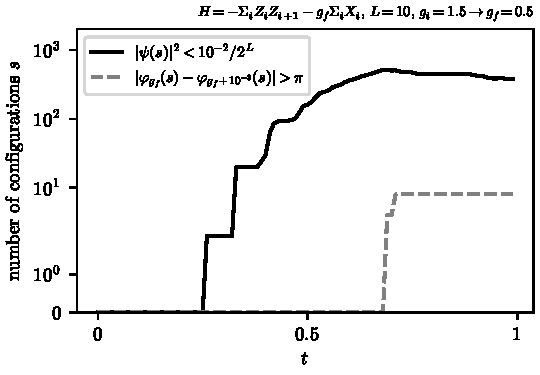
\includegraphics[width=0.46\linewidth]{fragility.pdf}
  \caption{Near-zeros and fragile windings for the transverse-field Ising quench $g_i=1.5\to g_f=0.5$, $L=10$, on the time grid of spacing $0.01$. Black: number of configurations $s$ (out of $2^L=1024$) with $|\psi(s,t)|^2<10^{-2}/2^L$, i.e.\ at least $100$ times below the uniform weight. Grey dashed: number of configurations whose time-continuous phase $\varphi(s,t)$ differs by more than $\pi$ between the quenches to $g_f=0.5$ and $g_f=0.501$, i.e.\ whose winding flipped. Symmetric-logarithmic vertical axis.}
  \label{fig:fragility}
\end{figure}

\begin{figure}[t]
  \centering
  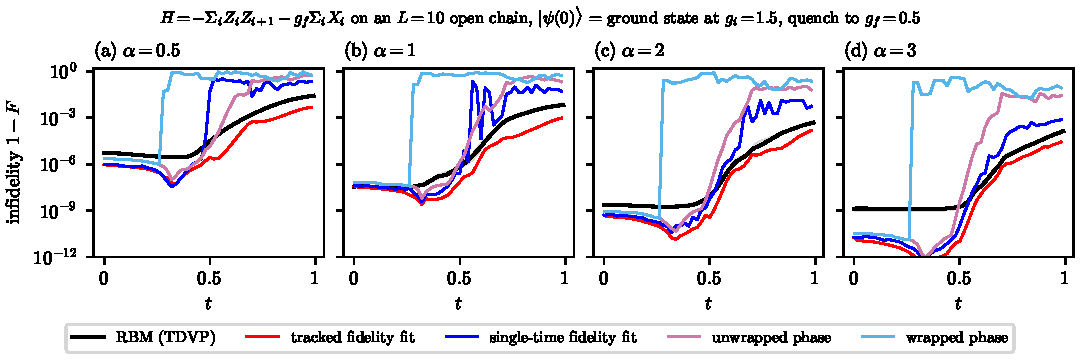
\includegraphics[width=\linewidth]{inf_vs_t_gf0.5.pdf}
  \caption{Infidelity of $K$-term cumulant models and of the RBM along the quench $g_i=1.5\to g_f=0.5$, $L=10$. Panels: RBM hidden-unit density $\alpha$, with $K=\alpha L^2+\alpha L+L$ cumulant terms. Black: RBM TDVP infidelity (median over five trials; grey band: min to max). Red: tracked fidelity fit. Dark blue: single-time fidelity fit. Pink: largest $K$ coefficients of $\log\psi$ with time-continuous phase. Light blue: same with the phase folded into $(-\pi,\pi]$. Values below $10^{-12}$ are clipped.}
  \label{fig:main}
\end{figure}

\section{Fitting the coefficients and tracking them in time}\label{sec:tracked}
\emph{A fidelity fit avoids the branch problem. Done at each time separately it is erratic once near-zeros appear; continued from one time step to the next, it ranks the RBM infidelity correctly, a factor of a few below it.}

\paragraph{Single-time fit.} The fidelity weights each configuration by $|\psi(s)|^2$, so near a near-zero the model only has to be small, not reproduce $\log\psi$. Fitting $\psi_K$ to $\psi$ directly therefore removes both the branch ambiguity and the logarithmic singularities. Up to $t\approx0.5$ this \fidfit{} is slightly better than the unwrapped phase (dark blue in \cref{fig:main}); after that it jumps erratically between times, reaching $5\times10^{-2}$ at $t=0.8$, $\alpha=1$, where the RBM has $1.8\times10^{-3}$ and the tracked fit below $10^{-4}$, with the same $K$. At $t=0.8$ this gap comes mainly from the support the single-time fit selects, not from local optima in $c_A$ or from the cumulant model (\cref{app:tracked}).

\paragraph{Tracked fit.}
 The \tracked{} imposes continuity in time on the coefficients $c_A(t)$ instead of on the phase $\varphi(s,t)$. This is analogous to TDVP, which also carries its parameters forward in time. Unlike TDVP, it is refit to the exact $\ket{\psi(t)}$ at every step. The resulting curves (red in \cref{fig:main}) follow the shape of the RBM curves for all four $\alpha$, including the onset of growth near $t\approx0.5$ and the ordering in $\alpha$. Above the RBM floor (\cref{fig:metrics}; individual points in \cref{app:gf}):
\begin{itemize}
  \item \textbf{Ranking in time and $\alpha$.} At $g_f=0.5$ the rank correlation is $\rho=0.98$, compared with $0.87$ for the unwrapped phase and $0.39$ for the wrapped phase. Within each of the six quenches it is $0.92$--$0.99$.
  \item \textbf{Ranking across runs.} The fixed-time rank correlation $\rho_t$ across the $24$ runs is $0.93$, against $0.76$ for the unwrapped phase and $0.89$ for the single-time fidelity fit. The tracked fit thus orders the runs by difficulty, not only the times.
  \item \textbf{Offset.} The tracked fit lies below the RBM, by a median factor of $5.6$ at $g_f=0.5$ and $3.7$ over all quenches.\footnote{The spread of $\log_{10}(\text{model}/\text{RBM})$ around its mean is $0.27$ decades at $g_f=0.5$ and $0.62$ decades over all quenches.}
\end{itemize}
The offset $\Delta$ varies between quenches, from a factor of $1.7$ ($g_f=3$) to $27$ ($g_f=0.3$), which is why the tracked fit does not predict the absolute RBM infidelity (\cref{fig:metrics}c). Its gain over the unwrapped phase is largest for $g_f=0.5$ and $0.7$, the quenches with the most near-zeros (\cref{fig:metrics}d). For $g_f\ge2$ there are no near-zeros, and the two nearly coincide.

Why the tracked fit beats the RBM was not established. One possible reason is that TDVP errors accumulate in time, while the tracked fit sees the exact state at every step. The other is a genuine difference in what RBMs and cumulant models can represent (see Limitations).

\begin{finding}[: the tracked fidelity fit ranks the RBM infidelity]
The \tracked{} reproduces the ordering of the RBM infidelity in time and $\alpha$ ($\rho=0.98$ at $g_f=0.5$) and across runs at fixed time ($\rho_t=0.93$), the best of the six models. It lies a factor of $1.7$ to $27$ below the RBM, depending on the quench, so it predicts relative, not absolute, RBM accuracy.
\end{finding}

\begin{figure}[t]
  \centering
  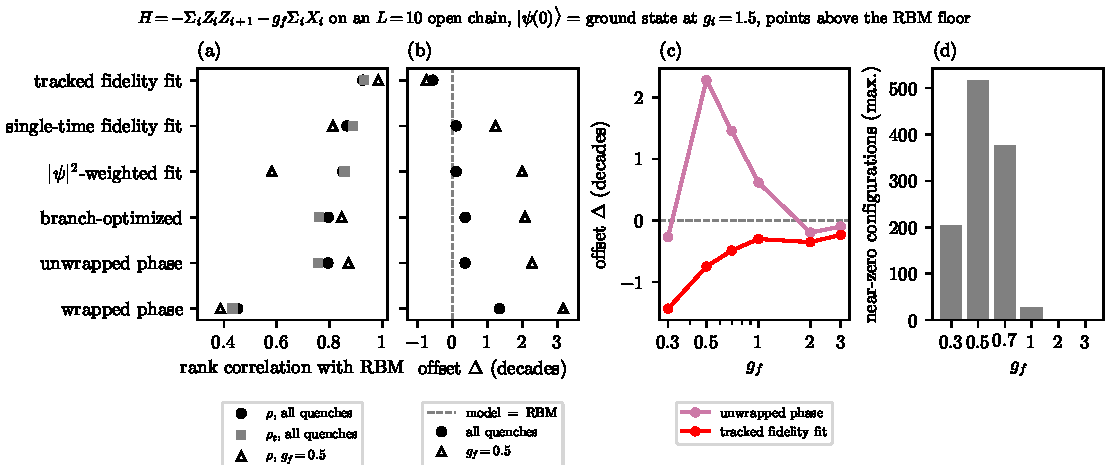
\includegraphics[width=\linewidth]{metrics.pdf}
  \caption{Agreement of the cumulant models with the RBM TDVP infidelity, using only points above the RBM floor (RBM infidelity more than $10$ times its $t=0$ value). (a) Rank correlations: Spearman $\rho$ pooled over times, $\alpha$ and all six quenches (black dots) or at $g_f=0.5$ only (open triangles); fixed-time rank correlation $\rho_t$ across the $24$ runs, averaged over time (grey squares). (b) Offset $\Delta$, the median of $\log_{10}(\text{model}/\text{RBM})$, markers as in (a); dashed: model equals RBM. (c) Offset $\Delta$ per quench $g_f$ for the unwrapped phase (pink) and the tracked fidelity fit (red). (d) Largest number of near-zero configurations ($|\psi(s)|^2<10^{-2}/2^L$) over $0\le t\le0.99$. Exact values are listed in \cref{app:tables}.}
  \label{fig:metrics}
\end{figure}

\section{Truncation curves: the RBM's own cumulants spread out}\label{sec:trunc}
\emph{Up to $t\approx0.5$ the top-$N_\mathrm{trunc}$ truncation behaves as for ground states. Later, neither the exact state's nor the RBM state's logarithm can be truncated to $N_\mathrm{var}$ terms, even though the full RBM state is much more accurate (most clearly for $\alpha\ge2$).}

\Cref{fig:trunc} repeats the analysis of Fig.~6 of Ref.~\cite{Cortes25} along the quench to $g_f=0.5$. For a given $\log\psi$, keep $c_\emptyset$ and the $N_\mathrm{trunc}$ largest $|c_A|$, exponentiate, and compute the infidelity with the exact $\ket{\psi(t)}$. The grey curve truncates the exact state's logarithm with time-continuous phase. The coloured curves truncate the RBM state's logarithm and approach its full infidelity as $N_\mathrm{trunc}\to2^L$. They use either the network's own branch, $\log\psi_\mathrm{RBM}=\sum_i a_is_i+\sum_j\log\cosh\theta_j(s)$ (top row, \emph{network branch}; $\theta_j(s)=b_j+\sum_iW_{ji}s_i$ with RBM weights $a_i,b_j,W_{ji}$), or the RBM phase made continuous in time (bottom row). The cumulant models of \cref{sec:fail,sec:tracked} have $K=N_\mathrm{var}$ terms, so $N_\mathrm{trunc}=N_\mathrm{var}$ is the point of comparison. These RBM states come from a new TDVP run that stores the states.\footnote{Same protocol as the earlier runs plus an L-BFGS refinement of the initial fit. For $\alpha=3$ the adaptive RK45 integrator stalled near $t=0$, so this run uses fixed-step RK4 with time step $\delta t=2.5\times10^{-4}$. For $t\ge0.5$ the new infidelities agree with the earlier runs to within a factor of about $2$ ($\alpha\le2$) and $3$ ($\alpha=3$).}
\begin{itemize}
  \item \textbf{$t\le0.3$.} As for ground states, each RBM curve follows the exact-state (grey) curve until it plateaus at the RBM infidelity. At the RBM parameter count $N_\mathrm{var}$, the exact-state curve lies below the RBM,\footnote{By factors $1$--$3$ for $\alpha=1$, $3$--$70$ for $\alpha=0.5$ and $2$, and $2$--$3$ orders of magnitude for $\alpha=3$.} whose plateau is set by its initial fit.
  \item \textbf{$t=0.5$.} The exact-state curve at $N_\mathrm{var}$ is within a factor of $2.5$ of the RBM for all four $\alpha$.\footnote{$1.4\times10^{-5}$, $1.4\times10^{-6}$, $3.1\times10^{-8}$, $3.7\times10^{-9}$ against $3.2\times10^{-5}$, $6.4\times10^{-7}$, $2.0\times10^{-8}$, $6.2\times10^{-9}$ for $\alpha=0.5,1,2,3$.} For $\alpha=2$, however, the network's own branch truncated to $N_\mathrm{var}$ terms gives $3\times10^{-2}$; its curve reaches the plateau only near $N_\mathrm{trunc}\approx400$. With the time-continuous RBM phase the same state gives $2.3\times10^{-8}$. The network branch is thus not the compressible one. We attribute this, without having checked it, to the branch cut of $\log\cosh\theta_j$, which makes the phase jump between configurations where $\cosh\theta_j(s)$ lies near the negative real axis.
  \item \textbf{$t\ge0.7$.} The exact-state curve stays above $10^{-2}$ up to $N_\mathrm{trunc}=300$ and falls below $10^{-4}$ only beyond $N_\mathrm{trunc}\approx500$. At $N_\mathrm{var}$ it overshoots the RBM by one to four orders of magnitude ($6\times10^{-2}$ against $7.6\times10^{-6}$ for $\alpha=2$, $t=0.7$). The RBM's own curves behave similarly under either branch: truncated to $N_\mathrm{var}$ terms they are $0.4$ to $3.5$ orders of magnitude worse than the full RBM state, most for $\alpha\ge2$.\footnote{At $t=0.7$, network branch: $1.0$, $0.8$, $3.5$, $2.2$ decades for $\alpha=0.5,1,2,3$; continuous phase: $0.8$, $1.2$, $2.0$, $3.2$. At $t=0.9$: $0.5$, $0.4$, $2.1$, $2.6$ and $1.0$, $0.7$, $1.1$, $2.8$.} The tracked fit (stars) stays at or below the RBM plateau.
\end{itemize}
For the ground states of Ref.~\cite{Cortes25}, the RBM's cumulant spectrum is concentrated in about $N_\mathrm{var}$ terms, which is why the top-$N_\mathrm{var}$ truncation predicts its accuracy. After $t\approx0.5$ this concentration is lost for the RBM state as well. The RBM's $\log\cosh$ terms stay a compact parametrization of a $\log\psi$ whose coefficients are not compact. We read this as the reason no branch of $\log\psi$ restored the top-$N$ predictor (\cref{sec:fail}), while a fidelity fit with the same $K$ can reach the RBM's accuracy (\cref{sec:tracked}). One caveat for the bottom row: between stored times, the RBM phase changes by close to $\pi$ at some configurations for $\alpha\ge1$,\footnote{By up to $2.7$, $3.1$ and $3.1$ rad for $\alpha=1$, $2$ and $3$, with stored times spaced by $10^{-3}$.} so the time-continuous RBM phase is likely ambiguous at a few near-zero configurations late in the evolution.

\begin{finding}[: top-$N$ truncation fails for the RBM state too]
After $t\approx0.5$, truncating even the RBM state's own $\log\psi$ to the RBM parameter count $N_\mathrm{var}$ makes its infidelity $0.4$ to $3.5$ orders of magnitude worse, on either branch and most for $\alpha\ge2$. The full RBM state is much more accurate than its truncated cumulant expansion, which we read as the reason no branch restored the ground-state predictor.
\end{finding}

\begin{figure}[t]
  \centering
  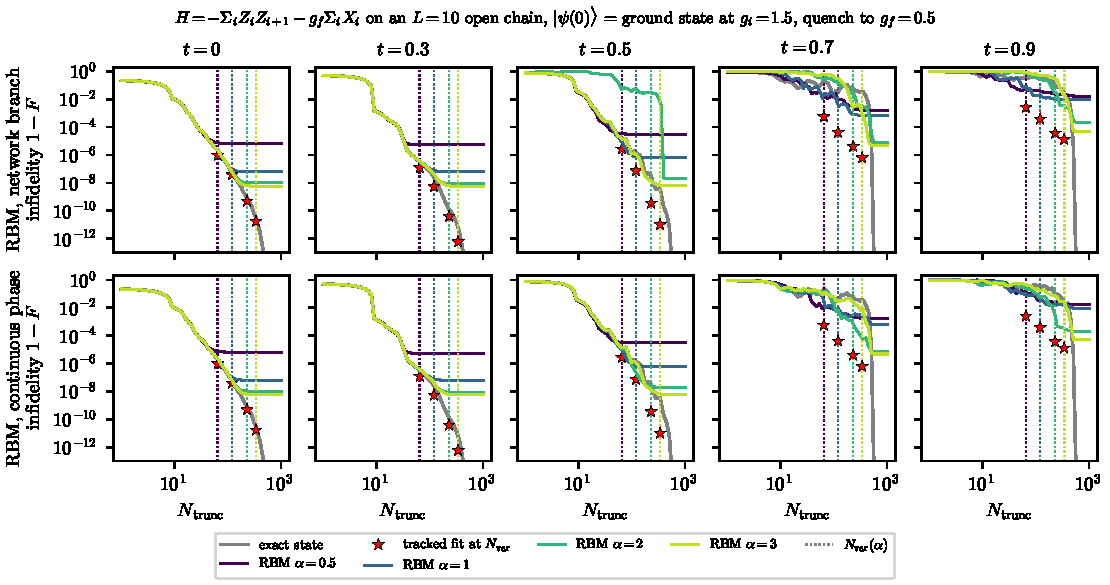
\includegraphics[width=\linewidth]{truncation_vs_N.pdf}
  \caption{Infidelity with the exact state $\psi(t)$ of the top-$N_\mathrm{trunc}$ cumulant truncation, along the quench $g_i=1.5\to g_f=0.5$, $L=10$; columns are times $t$. Grey: truncation of the exact $\log\psi$ with time-continuous phase. Coloured lines: truncation of the RBM TDVP state's $\log\psi$, coloured by hidden-unit density $\alpha$ (here the RBM is not black); at $N_\mathrm{trunc}=2^L-1$ they equal the RBM infidelity. Top row: the network branch, $\sum_ia_is_i+\sum_j\log\cosh\theta_j(s)$. Bottom row: RBM phase made continuous in time on a grid of spacing $10^{-3}$. Dotted: $N_\mathrm{var}(\alpha)$, coloured by $\alpha$. Red stars: tracked fidelity fit with $K=N_\mathrm{var}$ terms (\cref{sec:tracked}). Values below $10^{-13}$ are clipped.}
  \label{fig:trunc}
\end{figure}

\section{Verdict}
\begin{itemize}
  \item \textbf{Can a branch choice restore the cumulant predictor?} Only partly. Time-continuous unwrapping removes the $2\pi$ wrapping failure, and is exact for the classical quench. It fails once configurations approach zero amplitude. For the branches we tried, their logarithm stays non-local in $s$, and the winding itself becomes fragile.
  \item \textbf{Remedy.} Define the truncated cumulant expansion variationally, as the $K$-term $\exp(\sum_A c_A s^A)$ of highest fidelity, and continue it in time. It needs no branch. Its rank correlation $\rho$ with the RBM infidelity does not degrade in the quenches with many near-zeros ($\rho\ge0.98$ for $g_f\le0.7$). At fixed time it orders the $24$ runs with $\rho_t=0.93$, the best of the six models.
  \item \textbf{Why top-$N$ fails.} After $t\approx0.5$ the RBM state's own cumulants are spread over many more than $N_\mathrm{var}$ terms, under either branch (\cref{fig:trunc}). The truncated expansion then no longer describes what the RBM represents.
  \item \textbf{Not an exact equivalence.} The tracked fit lies below the RBM by a factor that varies from $1.7$ to $27$ between quenches. It predicts the time and $\alpha$ dependence within a quench and the ordering of runs at fixed time, not the absolute RBM infidelity.
\end{itemize}

\paragraph{Limitations.}
\begin{itemize}
  \item One model and one size ($L=10$, open chain, $Z$ basis); rotated bases and larger systems were not tested.
  \item The tracked fit is a local optimization with a heuristic support search. A better optimizer could lower its infidelity and change the offset.
  \item The main open question: a supervised RBM fit to $\psi(t)$, continued in time like the tracked fit, would separate TDVP error from representability. It was not run.
  \item The truncation curves (\cref{fig:trunc}) use a single new TDVP run per $\alpha$, and the $\alpha=3$ run is sensitive to the time step.\footnote{With RK4 at $\delta t=10^{-3}$, its infidelity jumped by a factor of $10^3$ within one step at $t\approx0.6$; at $\delta t=2.5\times10^{-4}$ the largest one-step jump is a factor of $10$ (at $t=0.626$).}
  \item The tracked fit costs far more than a Walsh--Hadamard transform. It needs the exact state and a nonconvex optimization at every time step, so it is a diagnostic, not a cheap proxy.
\end{itemize}

\FloatBarrier
\appendix

\section{Notation}\label{app:notation}
\begin{center}
\small
\begin{tabular}{lll}
  \toprule
  symbol & meaning & defined in \\
  \midrule
  $L$ & number of spins ($L=10$) & \cref{sec:setup} \\
  $g_i$, $g_f$ & transverse field before and after the quench & \cref{sec:setup} \\
  $s$, $s^A$ & spin configuration; product of $s_i$ over the subset $A$ & \cref{sec:defs} \\
  $c_A$ & cumulant coefficient of $\log\psi$ & \cref{sec:defs} \\
  $\varphi(s)$ & phase of $\psi(s)$, made continuous in time where stated & \cref{sec:defs} \\
  $n(s)$, $\log_n\psi$ & winding number (branch) of the phase; logarithm on branch $n$ & \cref{sec:defs} \\
  near-zero & configuration with $|\psi(s)|^2<10^{-2}/2^L$ & \cref{sec:defs} \\
  $S$, $K$ & support and number of terms of the cumulant model & \cref{sec:defs} \\
  $\psi_K$ & $K$-term cumulant model & \cref{sec:defs} \\
  $\alpha$ & RBM hidden-unit density (hidden units $\alpha L$) & \cref{sec:defs} \\
  $N_\mathrm{var}$ & number of complex RBM parameters, $\alpha L^2+\alpha L+L$ & \cref{sec:defs} \\
  $1-F$ & infidelity with the exact state & \cref{sec:defs} \\
  $\rho$ & rank correlation with the RBM, pooled over times and $\alpha$ & \cref{sec:defs} \\
  $\rho_t$ & rank correlation across runs at fixed time & \cref{sec:defs} \\
  $\Delta$ & offset: median $\log_{10}(\text{model}/\text{RBM})$, in decades & \cref{sec:defs} \\
  $\chi$ & generic model state (cumulant model or RBM) & \cref{sec:defs} \\
  $N_\mathrm{trunc}$ & number of coefficients kept in a truncation & \cref{sec:trunc} \\
  $\theta_j(s)$ & input of RBM hidden unit $j$, $b_j+\sum_iW_{ji}s_i$ & \cref{sec:trunc} \\
  $\delta t$ & integrator time step of the RBM TDVP run & \cref{sec:trunc} \\
  $\phi$, $\mathcal{L}$ & model with free coefficients; objective $-\log F$ & \cref{app:tracked} \\
  $p(s)$, $m(s)$ & model's probability distribution; overlap weighting & \cref{app:tracked} \\
  $G_A$ & score of a candidate term $A$ (size of the fidelity gradient) & \cref{app:tracked} \\
  \bottomrule
\end{tabular}
\end{center}

\section{Method details}\label{app:methods}
\begin{itemize}
  \item \textbf{Branch-optimized.} Alternate between (i) the largest $K$ coefficients of $\log_n\psi$ and (ii) $n(s)\leftarrow\mathrm{round}\bigl[(\mathrm{Im}\log\psi_K(s)-\varphi(s))/2\pi\bigr]$. Each step lowers $\sum_s|\log_n\psi(s)-\log\psi_K(s)|^2$; iterate until $n$ stops changing.
  \item \textbf{$|\psi|^2$-weighted fit.} To second order in the error, $1-F$ equals the $|\psi|^2$-weighted variance of $\log\psi_K-\log\psi$. We minimize $\sum_s|\psi(s)|^2|\log_n\psi(s)-\log\psi_K(s)|^2$ with the support grown greedily (orthogonal matching pursuit, batches of $K/20$ subsets), followed by the winding update above; three rounds.
  \item \textbf{Single-time fidelity fit.} Minimize $-\log F$ over the real and imaginary parts of $c_A$, $A\in S$, with the analytic gradient (L-BFGS, \texttt{scipy}).
  \item \textbf{Tracked fidelity fit.} At each time: (i) fidelity fit from the previous $(S,c)$; (ii) two swap rounds, each adding the $K/10$ subsets with the largest fidelity gradient, refitting, removing the $K/10$ smallest $|c_A|$ and refitting, kept only if the infidelity decreases; (iii) a fresh $|\psi|^2$-weighted plus fidelity fit, kept instead if better. The first step at $t=0$ is a fresh fit. Derivation, diagnostics and ablations are in \cref{app:tracked}.
  \item \textbf{Time grid.} The cumulant models are evaluated at every second point of the RBM grid, $t=0,0.02,\dots,0.98$. The near-zero and winding counts (\cref{fig:fragility,fig:metrics}) use the full grid of spacing $0.01$.
\end{itemize}

\FloatBarrier
\section{The tracked fidelity fit in detail}\label{app:tracked}
\emph{The tracked fit looks for the $K$-term cumulant model that is closest to the exact state, as measured by the fidelity, and follows this model from one time step to the next. It works mainly because it keeps a good choice of which $K$ terms to use.}

\subsection{The idea in brief}
The cumulant model writes the wave function as the exponential of a sum of $K$ spin products with complex coefficients. The ground-state recipe of Ref.~\cite{Cortes25} picks the terms and their coefficients from $\log\psi$: it keeps the $K$ largest coefficients of its expansion in spin products. In a quench this runs into two problems (\cref{sec:fail}). The imaginary part of $\log\psi$, the phase, is defined only up to multiples of $2\pi$. And at configurations whose amplitude passes close to zero, $\log\psi$ becomes large and changes abruptly. The tracked fit never takes the logarithm of $\psi$:
\begin{enumerate}
  \item It chooses the $K$ terms and their coefficients so that the exponential of the model has the largest possible overlap (fidelity) with $\psi(t)$. Only $\psi$ itself enters, never $\log\psi$.
  \item At the next time step it starts from the terms and coefficients found at the previous step. Since $\psi$ changes little within one step, the previous solution is already close to the new one.
  \item At each step it tries to exchange a few of the kept terms for better ones, proposing the terms that would improve the fidelity fastest.
\end{enumerate}
A picture: the fidelity defines a landscape over all possible coefficient values, and the best model sits in a valley. As time goes on the landscape changes shape. The tracked fit follows the valley it started in at $t=0$, where the problem is easy, instead of searching the whole landscape anew at every time.

All examples below are for the quench $g_i=1.5\to g_f=0.5$ with $K=120$ terms, as many as the complex parameters of an RBM with $\alpha=1$, on the time grid $t=0,0.02,\dots,0.98$.

\begin{definition}[: quantities used in this appendix]
\begin{itemize}
  \item \textbf{Configurations.} $s=(s_1,\dots,s_L)$ with $s_i=\pm1$; for $L=10$ there are $2^L=1024$ of them. The exact amplitude $\psi(s)$ is known for each.
  \item \textbf{Terms.} For a set of sites $A$, $s^A=\prod_{i\in A}s_i$ is the product of those spins, e.g.\ $s^{\{4,5\}}=s_4s_5$. A term is $c_As^A$ with a complex coefficient $c_A$. The \emph{order} $|A|$ of a term is the number of spins in the product.
  \item \textbf{Model.} $\phi(s)=\exp\bigl(\sum_{A\in S}c_As^A\bigr)$. The set of kept terms $S$ contains the constant term ($A=\emptyset$, which only sets the norm and global phase) and $K$ others.
  \item \textbf{Fidelity.} $F=|\braket{\psi|\phi}|^2/(\braket{\psi|\psi}\braket{\phi|\phi})$, between $0$ and $1$; $1-F$ is the infidelity.
  \item \textbf{Near-zero.} A configuration whose probability $|\psi(s)|^2$ is more than $100$ times below the uniform value $1/2^L$.
\end{itemize}
\end{definition}

\subsection{What is optimized, and why the phase problem disappears}
The fit minimizes $\mathcal{L}=-\log F$ over the real and imaginary parts of the coefficients $c_A$ of the kept terms. Minimizing $-\log F$ is the same as maximizing $F$, but it is better behaved numerically when $F$ is close to $1$. Two properties make this objective immune to the problems of $\log\psi$:
\begin{itemize}
  \item \textbf{Phase ambiguities are invisible.} The fidelity compares $\phi$ and $\psi$ themselves. Adding $2\pi$ to the phase of $\phi(s)$ at any configuration leaves $\phi$, and hence $F$, unchanged. A fit of $\log\psi$ instead counts such a $2\pi$ mismatch as a large error, unless the phase of $\psi$ has been continued in exactly the matching way.
  \item \textbf{Near-zero configurations matter little.} With both states normalized ($\hat\psi$, $\hat\phi$) and the best global phase $\theta$ between them,
  \[
    \sum_s\bigl|\hat\psi(s)-e^{i\theta}\hat\phi(s)\bigr|^2=2\bigl(1-\sqrt F\bigr)\approx1-F .
  \]
  The infidelity is thus a sum of squared amplitude differences, one per configuration. At a near-zero, $\hat\psi(s)\approx0$ and the contribution is simply $|\hat\phi(s)|^2$: the model only has to be small there, and the value of its logarithm, or of its phase, is irrelevant. A fit of $\log\psi$, in contrast, has to reproduce the deep dip of $\log|\psi|$ and the rapid turn of the phase at every near-zero.
\end{itemize}
The coefficients keep one harmless ambiguity. Since $s^A=\pm1$, adding $i\pi$ to a single coefficient $c_A$ multiplies $\phi$ by $-1$ at every configuration, which is only a global sign. So the imaginary part of each coefficient matters only up to multiples of $\pi$, and the constant term does not matter at all. This is the phase ambiguity in another guise, but it never has to be resolved, because all these choices give the same $\phi$.

\subsection{How the fit decides which terms to add}
To improve the model we need to know which terms not yet kept would help most. The derivative of $\mathcal{L}$ with respect to their coefficients answers this. It involves two weightings of the configurations,
\[
  p(s)=\frac{|\phi(s)|^2}{\braket{\phi|\phi}},\qquad m(s)=\frac{\psi^*(s)\phi(s)}{\braket{\psi|\phi}} .
\]
Here $p$ is the probability distribution of the model, and $m$ is a complex weighting built from the overlap of model and exact state (it sums to $1$ but need not be positive). Write $\braket{s^A}_p=\sum_sp(s)s^A$ for the average of the product $s^A$ under $p$, and similarly for $m$. Because $\phi$ is an exponential, $\partial\phi(s)/\partial c_A=s^A\phi(s)$, and the norm $\braket{\phi|\phi}$ depends only on the real parts of the coefficients. This gives
\[
  \frac{\partial\mathcal{L}}{\partial\,\mathrm{Re}\,c_A}=2\bigl(\braket{s^A}_p-\mathrm{Re}\braket{s^A}_m\bigr),\qquad
  \frac{\partial\mathcal{L}}{\partial\,\mathrm{Im}\,c_A}=2\,\mathrm{Im}\braket{s^A}_m .
\]
In words:
\begin{itemize}
  \item \textbf{At the best coefficients}, every kept spin product has the same average under both weightings: $\braket{s^A}_m=\braket{s^A}_p$ for all $A\in S$. If $\phi$ equals $\psi$, both weightings reduce to $|\psi|^2$ and the condition holds trivially.\footnote{For the tracked fit at $t=0.8$, the two averages differ by at most $1.1\times10^{-8}$ for kept terms, and by up to $4.8\times10^{-4}$ for terms not kept.}
  \item \textbf{For a term not yet kept} ($c_A=0$), the size of the gradient,
  \[
    G_A=2\bigl|\braket{s^A}_p-\braket{s^A}_m\bigr| ,
  \]
  is the rate at which $\mathcal{L}$ would start to decrease if this term were switched on. It is the score used to propose new terms. The averages for all $2^L$ possible terms come out of one fast Walsh--Hadamard transform each of $p$ and $m$, the same transform that gives the cumulant coefficients.
\end{itemize}

\subsection{The procedure step by step}
\begin{enumerate}
  \item \textbf{Start ($t=0$).} The initial ground state is real and positive, so its logarithm poses no problem. The terms are chosen by a least-squares fit of $\log\psi(0)$ weighted by $|\psi(0)|^2$, adding terms greedily in batches of $K/20$. The coefficients are then refined by maximizing the fidelity.
  \item \textbf{Each later time step} ($\Delta t=0.02$):
  \begin{enumerate}
    \item \emph{Refit from the previous solution.} Keep the same terms, start from the previous coefficients, and maximize the fidelity with the new $\psi(t)$.
    \item \emph{Exchange terms}, two rounds. Propose the $K/10$ terms (here $12$) with the largest score $G_A$. Fit with these $K+12$ terms, the new coefficients starting at zero. Discard the $12$ terms with the smallest $|c_A|$ and refit. Accept the exchange only if the fidelity improved.
    \item \emph{Safety net.} Also fit from scratch at this time, as in step 1, and keep that result if it is better.
  \end{enumerate}
\end{enumerate}
All fits use L-BFGS, a standard gradient-based optimizer, with the exact gradient above. For $K=120$, a complete run over the $50$ time steps takes about $3$ minutes on one core. Two remarks:
\begin{itemize}
  \item Discarding the terms with the smallest $|c_A|$ is a rule of thumb: a small coefficient does not guarantee a small loss of fidelity.
  \item As implemented, the from-scratch fit of step 2(c) starts from the phase folded into $(-\pi,\pi]$. It fails once phases leave this interval at $t=0.28$ (grey dashed in \cref{fig:tr-ablation}a), and here it never won after $t=0$. In practice the tracked fit therefore consists of steps 2(a) and 2(b); leaving out 2(c) gives identical results.
\end{itemize}

\subsection{Comparison with RBM time evolution}
The RBM curves come from the time-dependent variational principle (TDVP). Like the tracked fit, TDVP starts from a fit of the initial state and moves its parameters continuously in time. Two differences matter:
\begin{itemize}
  \item TDVP never sees the exact state at later times. It moves the parameters in the direction that best follows the Schrödinger equation, so errors made early on are carried forward. The tracked fit is compared with the exact $\psi(t)$ at every step, so its errors do not accumulate.
  \item The tracked fit may change which terms it uses; the structure of an RBM is fixed.
\end{itemize}
The tracked fit is therefore closer to fitting the model directly to the known exact state at each time. Its infidelity is an upper bound on the best infidelity any $K$-term cumulant model can reach at that time, though not necessarily a tight one.

\subsection{What the diagnostics show}
Each paragraph below answers one question.

\paragraph{Which ingredients matter? (\cref{fig:tr-ablation}a)} We switched off parts of the procedure one at a time.
\begin{itemize}
  \item \emph{Keeping the $t=0$ terms} and updating only their coefficients is nearly as good up to $t\approx0.45$ (within a factor of $2.5$), but falls behind later. At $t=0.8$ it gives $7.4\times10^{-4}$, $7.5$ times worse than the full tracked fit ($9.9\times10^{-5}$), though still $2.4$ times below the RBM ($1.8\times10^{-3}$).
  \item \emph{Fitting from scratch at each time} (the single-time fit: same objective, no memory of earlier times) becomes erratic from $t=0.56$ and reaches $4.7\times10^{-2}$ at $t=0.8$. Started from the folded phase, it fails already at $t=0.28$.
\end{itemize}

\paragraph{How much do the exchanges of terms do? (\cref{fig:tr-ablation}b,c)} Over the $49$ steps, $131$ terms are exchanged, mostly between $t=0.25$ and $0.7$ and up to $14$ in one step. Each step's exchanges improve the infidelity only slightly (median factor $1.02$, largest $2.3$ at $t=0.34$). The improvements add up, however: without exchanges the infidelity at $t=0.8$ is $7.5$ times higher.

\paragraph{Which terms are kept? (\cref{fig:tr-coeffs}a)} At $t=0$ the model keeps all $45$ two-spin products, $74$ of the $210$ four-spin products and one six-spin product. Six-spin products enter from $t\approx0.45$, when the infidelity starts to grow; at $t=0.8$ the model keeps $37$ two-spin, $67$ four-spin and $16$ six-spin terms. Products of an odd number of spins never appear. The Hamiltonian and the initial state are unchanged when all spins are flipped, so $\psi(s)=\psi(-s)$ and odd products drop out.

\paragraph{Do the coefficients change smoothly? (\cref{fig:tr-coeffs}b,c)} For the tracked fit they do, even after $t\approx0.5$, when the phase of many configurations becomes ill-defined. The single-time fit gives the same coefficients up to $t\approx0.55$; after that they jump from step to step, with magnitudes up to $8.6$ against at most $0.94$ for the tracked fit. These jumps are genuine differences, not the harmless $i\pi$ ambiguity: they also occur in the real parts, and the jumps in the imaginary parts are not multiples of $\pi$.

\paragraph{Where does the remaining error come from? (\cref{fig:tr-mech}a,b)} At $t=0.8$ the tracked fit's error per configuration is roughly the same for likely and unlikely configurations. More than half of its total error ($57\%$) comes from the $450$ near-zeros, which together hold only $0.1\%$ of the probability. The truncation of $\log\psi$ with unwrapped phase ($1-F=0.37$) does the opposite: its error is largest at the most likely configurations, and near-zeros account for only $0.2\%$ of it. Truncating in log space thus turns a problem at a few unimportant configurations into errors at the important ones.

\paragraph{Is it the choice of terms or the starting coefficients? (\cref{fig:tr-mech}c)} We refit at $t=0.8$ with the set of terms held fixed, from several starting coefficients.
\begin{itemize}
  \item With the tracked fit's terms, starting from all coefficients zero (a uniform state) reaches the same infidelity, $9.9\times10^{-5}$, as starting from the previous time step. Starting from a weighted fit of $\log\psi$ ends in a worse local minimum ($4.8\times10^{-4}$). Starting from the single-time fit's coefficients gets stuck at $2.8\times10^{-2}$.
  \item With the single-time fit's terms, which share only $49$ of $121$ with the tracked fit, no start goes below $4.7\times10^{-2}$, not even the tracked fit's coefficients.
\end{itemize}
Which terms are kept is thus what matters; the starting coefficients matter only when they are far off. The single-time fit chooses its terms by fitting $\log\psi$, which requires a choice of phase branch, and we attribute its poor choice at late times to the windings and dips of $\log\psi$ at near-zeros. The tracked fit chooses its terms at $t=0$, where this is easy, and then adjusts a few at a time.

\begin{finding}[: tracking works by keeping good terms]
With the terms carried forward by the \tracked{}, a fit at $t=0.8$ reaches $1-F=9.9\times10^{-5}$ even from zero coefficients; with the terms chosen by the \fidfit{}, no start goes below $4.7\times10^{-2}$. Following the solution in time supplies these terms: they are chosen at $t=0$ and adjusted a few at a time along the fidelity gradient. Each exchange gains little, but together they gain a factor of $7.5$ by $t=0.8$.
\end{finding}

\paragraph{Caveats.} The tracked solution is not guaranteed to be the best possible $K$-term model: terms are exchanged greedily and each fit finds only a nearby optimum. The time step $0.02$ was not varied. These diagnostics are shown only for $g_f=0.5$ and $\alpha=1$; the statistics in the main text cover all quenches and $\alpha$.

\begin{figure}[tbp]
  \centering
  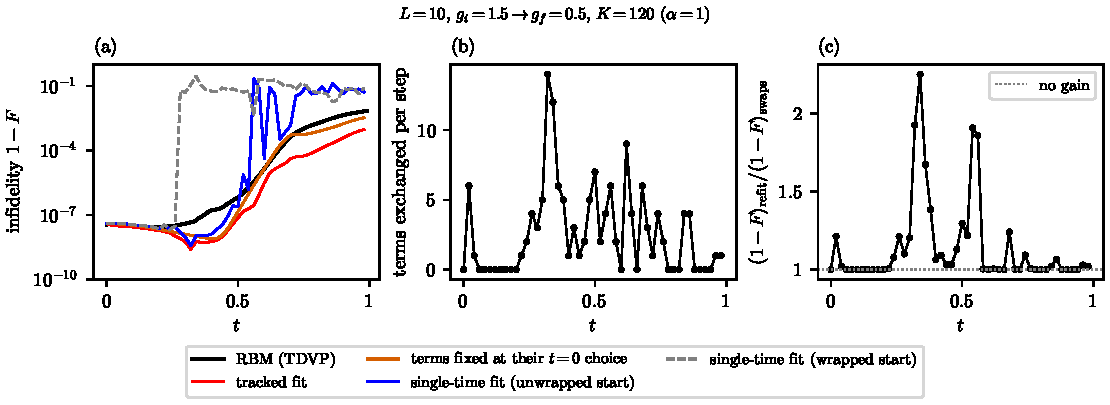
\includegraphics[width=\linewidth]{tracked_ablation.pdf}
  \caption{Variants of the tracked fidelity fit with ingredients switched off, for the quench $g_i=1.5\to g_f=0.5$, $L=10$, $K=120$ terms ($\alpha=1$). (a) Infidelity with the exact state. Black: RBM time evolution (TDVP, median over five trials). Red: tracked fit. Orange: terms kept fixed at their $t=0$ choice, only coefficients updated. Blue: fit from scratch at each time (single-time fit), started from a fit of $\log\psi$ with phase continuous in time, as in the main text. Grey dashed: the same, started from the phase folded into $(-\pi,\pi]$; this is the safety net inside the tracked fit. The tracked fit without the safety net coincides with the red curve and is not drawn. (b) Number of terms exchanged between consecutive time steps ($\Delta t=0.02$). (c) Infidelity after refitting the previous step's terms, divided by the infidelity after the exchanges; dotted: no gain.}
  \label{fig:tr-ablation}
\end{figure}

\begin{figure}[tbp]
  \centering
  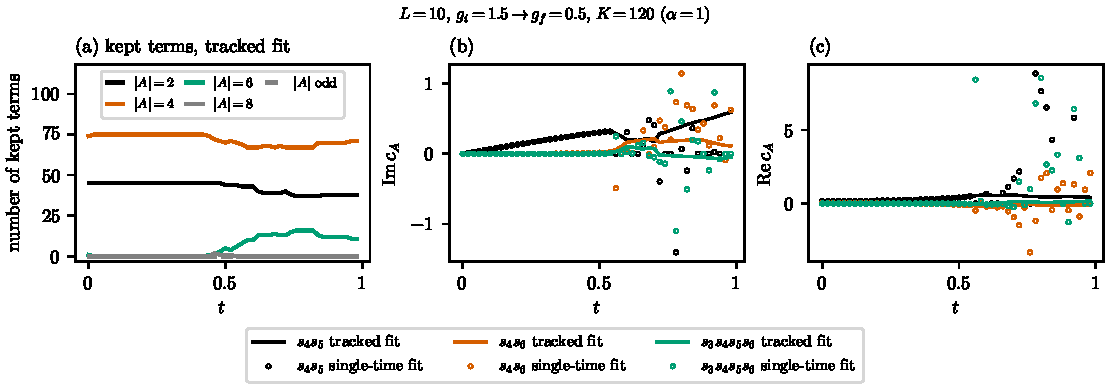
\includegraphics[width=\linewidth]{tracked_coeffs.pdf}
  \caption{Terms and coefficients of the tracked fidelity fit for the quench $g_i=1.5\to g_f=0.5$, $L=10$, $K=120$ ($\alpha=1$). (a) Number of kept terms by order $|A|$, the number of spins in the product; odd orders never occur. (b) Imaginary and (c) real parts of three coefficients: the central nearest-neighbour pair $s_4s_5$, the next-nearest-neighbour pair $s_4s_6$, and the four-spin product $s_3s_4s_5s_6$. Lines: tracked fit. Open circles: single-time fit. A coefficient whose term is not kept is plotted as zero. Here colours label terms, not methods.}
  \label{fig:tr-coeffs}
\end{figure}

\begin{figure}[tbp]
  \centering
  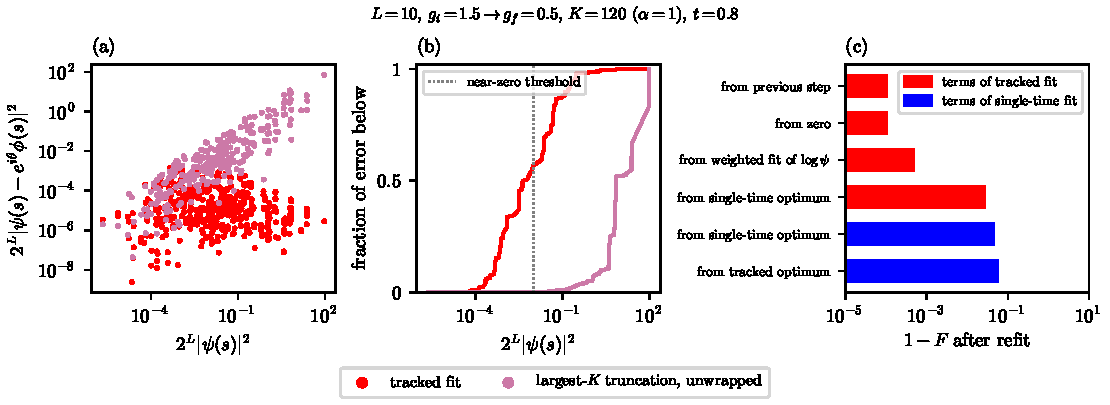
\includegraphics[width=\linewidth]{tracked_mechanism.pdf}
  \caption{Where the error sits at $t=0.8$, for the quench $g_i=1.5\to g_f=0.5$, $L=10$, $K=120$ ($\alpha=1$). (a) Error per configuration, $2^L|\hat\psi(s)-e^{i\theta}\hat\phi(s)|^2$ with both states normalized and the best global phase $\theta$, against the probability $2^L|\psi(s)|^2$ ($1$ is the uniform value). These errors sum to $2(1-\sqrt F)\approx1-F$. Red: tracked fit ($1-F=9.9\times10^{-5}$). Pink: largest $K$ coefficients of $\log\psi$ with phase continuous in time ($1-F=0.37$). (b) Fraction of the total error coming from configurations less likely than the abscissa; dotted: near-zero threshold. (c) Infidelity after a fit with the set of terms held fixed, from several starting coefficients. Red bars: terms of the tracked fit at $t=0.8$. Blue bars: terms of the single-time fit at $t=0.8$ ($49$ of $121$ shared). Starts: coefficients of the tracked fit at $t=0.78$ (previous step); all zero, i.e.\ a uniform state; a weighted least-squares fit of $\log\psi$; the coefficients of the other fit, with missing terms set to zero.}
  \label{fig:tr-mech}
\end{figure}

\FloatBarrier
\section{Agreement metrics: full tables}\label{app:tables}
\Cref{tab:methods,tab:gf} list the values plotted in \cref{fig:metrics}.

\begin{table}[h]
  \centering
  \caption{Agreement of each cumulant model with the RBM TDVP infidelity, for points above the RBM floor ($597$ points over all six quenches, $93$ at $g_f=0.5$). $\rho$: Spearman rank correlation pooled over times and $\alpha$ (and quenches). $\rho_t$: rank correlation across the $24$ runs at fixed time, averaged over time. $\Delta$: median of $\log_{10}(\text{model}/\text{RBM})$.}
  \label{tab:methods}
  \begin{tabular}{lccccc}
    \toprule
    & \multicolumn{3}{c}{all quenches} & \multicolumn{2}{c}{$g_f=0.5$} \\
    method & $\rho$ & $\rho_t$ & $\Delta$ & $\rho$ & $\Delta$ \\
    \midrule
    wrapped phase & 0.45 & 0.43 & $+1.34$ & 0.39 & $+3.17$ \\
    unwrapped phase & 0.79 & 0.76 & $+0.36$ & 0.87 & $+2.28$ \\
    branch-optimized & 0.80 & 0.76 & $+0.36$ & 0.85 & $+2.08$ \\
    $|\psi|^2$-weighted fit & 0.85 & 0.86 & $+0.10$ & 0.58 & $+1.99$ \\
    fidelity fit & 0.87 & 0.89 & $+0.10$ & 0.81 & $+1.23$ \\
    tracked fidelity fit & 0.93 & 0.93 & $-0.57$ & 0.98 & $-0.75$ \\
    \bottomrule
  \end{tabular}
\end{table}

\begin{table}[h]
  \centering
  \caption{Per-quench comparison of the tracked fidelity fit with the unwrapped phase, points above the RBM floor. $\rho$ (pooled over times and $\alpha$) and $\Delta$ as in \cref{tab:methods}. Near-zeros: largest number of configurations with $|\psi(s)|^2<10^{-2}/2^L$ over $0\le t\le0.99$ (time grid of spacing $0.01$).}
  \label{tab:gf}
  \begin{tabular}{ccccccc}
    \toprule
    & & & \multicolumn{2}{c}{unwrapped phase} & \multicolumn{2}{c}{tracked fidelity fit} \\
    $g_f$ & points & near-zeros & $\rho$ & $\Delta$ & $\rho$ & $\Delta$ \\
    \midrule
    0.3 & 69 & 204 & 0.99 & $-0.27$ & 0.99 & $-1.43$ \\
    0.5 & 93 & 516 & 0.87 & $+2.28$ & 0.98 & $-0.75$ \\
    0.7 & 96 & 376 & 0.87 & $+1.45$ & 0.98 & $-0.49$ \\
    1.0 & 93 & 28 & 0.90 & $+0.62$ & 0.93 & $-0.30$ \\
    2.0 & 97 & 0 & 0.95 & $-0.20$ & 0.95 & $-0.35$ \\
    3.0 & 149 & 0 & 0.92 & $-0.10$ & 0.92 & $-0.23$ \\
    \bottomrule
  \end{tabular}
\end{table}

\FloatBarrier
\section{Scatter for all quenches}\label{app:gf}
\Cref{fig:scatter} shows the individual points behind the pooled statistics of \cref{fig:metrics}.

\begin{figure}[h]
  \centering
  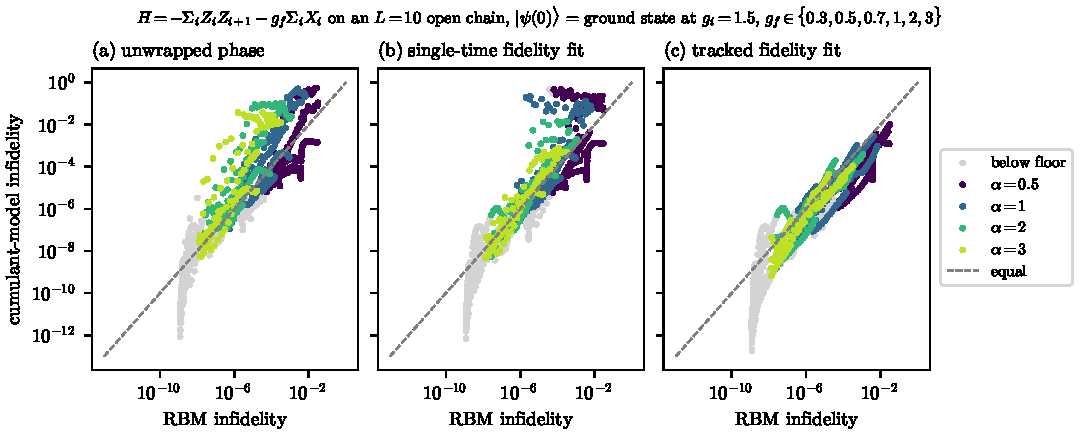
\includegraphics[width=\linewidth]{scatter_all.pdf}
  \caption{Cumulant-model infidelity against RBM TDVP infidelity (median of five trials) for all quenches $g_i=1.5\to g_f\in\{0.3,0.5,0.7,1,2,3\}$, $L=10$, and all times $0<t\le0.98$. Colour: RBM hidden-unit density $\alpha$ (cumulant terms $K=\alpha L^2+\alpha L+L$). Grey: points below the RBM floor (RBM infidelity at most $10$ times its $t=0$ value), excluded from the statistics. Dashed: equality. (a) Largest $K$ coefficients with time-continuous phase; (b) single-time fidelity fit; (c) tracked fidelity fit.}
  \label{fig:scatter}
\end{figure}

\section{Reproducibility}\label{app:repro}
\texttt{check\_time\_evolution/phase\_branch/phase\_branch.py} computes all cumulant models (\texttt{data/predictors.csv}). It also reads the RBM TDVP infidelities from the shared file \texttt{Inf\_RBM\_L10\_g1.5\_t1.0\_Ntimes100.pkl} into \texttt{data/rbm.csv}. \texttt{python phase\_branch.py --check} runs the self-checks (phase convergence, exact reconstruction, two-body phase at $g_f=0$). \texttt{make\_figs.py} writes \texttt{data/metrics.csv} and the figures. Run with one BLAS thread per process; the full run uses 24 processes for about 20 minutes. \texttt{rbm\_states.py} reruns RBM TDVP at $g_f=0.5$ and stores the states (\texttt{data/rbm\_states\_a*.npz}). Its initial infidelities are $6.5\times10^{-6}$, $6.4\times10^{-8}$, $1.0\times10^{-8}$ and $5.7\times10^{-9}$ for $\alpha=0.5,1,2,3$. \texttt{truncation.py} computes the truncation curves (\texttt{data/truncation.csv}). \texttt{tracked\_demo.py} reruns the tracked fit at $g_f=0.5$, $\alpha=1$ with its ablations (\texttt{data/tracked\_demo\_*.npz}) and checks that it reproduces \texttt{data/predictors.csv}; \texttt{tracked\_figs.py} makes \cref{fig:tr-ablation,fig:tr-coeffs,fig:tr-mech}.

\bibliographystyle{unsrt}
\bibliography{refs}
\end{document}
